% !TEX TS-program = xelatex
\documentclass[conference,a4paper]{IEEEtran}

\usepackage{fontspec}
\setmainfont{Times New Roman}
\setsansfont{Arial}
\setmonofont{Consolas}
\XeTeXlinebreaklocale "vi"
\XeTeXlinebreakskip = 0pt plus 1pt

\usepackage{amsmath}
\usepackage{booktabs}
\usepackage{graphicx}
\usepackage{hyperref}
\usepackage{xcolor}
\usepackage{listings}
\usepackage{float}
\usepackage{caption}
\usepackage{subcaption}
\usepackage{tikz}
\usetikzlibrary{positioning,arrows.meta,shapes.geometric,fit,backgrounds}

\hypersetup{colorlinks=true,linkcolor=blue,citecolor=green,urlcolor=magenta}

\title{Validation: OmniCast IEEE Template with Vietnamese diacritics}
\author{\IEEEauthorblockN{Test Author}\IEEEauthorblockA{Group OmniCast}}
\begin{document}
\maketitle
\begin{abstract}
Kiểm thử hiển thị tiếng Việt có dấu đầy đủ: nguyễn, đường, tiếng, Việt Nam, Đặng Thái Sơn, Ứng dụng, Phần mềm, triển khai, kiểm thử, hiệu năng, chất lượng, phụ thuộc, quản lý, đồng bộ, bảo mật, mã hóa, đăng nhập, đăng ký, lịch phát sóng, chương trình, chuyển kênh, gợi ý, tiện ích.
\end{abstract}
\begin{IEEEkeywords}
keyword one, keyword two, keyword three, hệ thống phát sóng, ứng dụng di động
\end{IEEEkeywords}

\section{Introduction}
Đây là đoạn văn tiếng Việt kiểm tra ngắt dòng và dấu thanh: nguyễn, Tiếng Việt, Đại học, Chuyên ngành, Thành phố Hồ Chí Minh, học kỳ, đồ án, phần mềm, hệ thống.

\section{Math and Table Test}
\begin{equation}
E = mc^2
\end{equation}

\begin{table}[H]
\caption{Test table}
\label{tab:test}
\begin{tabular}{lcc}
\toprule
Metric & Value & Unit \\
\midrule
Response time & 145 & ms \\
Throughput & 1200 & req/s \\
\bottomrule
\end{tabular}
\end{table}

\section{TikZ Test}
\begin{figure}[H]
\centering
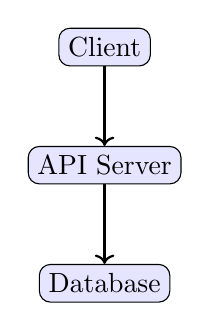
\begin{tikzpicture}[node distance=1.5cm, every node/.style={draw, rounded corners, fill=blue!10, align=center}]
\node (a) {Client};
\node (b) [below of=a] {API Server};
\node (c) [below of=b] {Database};
\draw[->, thick] (a) -- (b);
\draw[->, thick] (b) -- (c);
\end{tikzpicture}
\caption{Kiểm tra TikZ}
\end{figure}

\section{Listing Test}
\begin{lstlisting}[language=TypeScript,basicstyle=\ttfamily\small,caption={Code sample}]
export async function login(email: string, password: string) {
  const user = await prisma.user.findUnique({ where: { email } });
  if (!user) throw new UnauthorizedException('Sai thông tin');
  return this.jwt.sign({ sub: user.id, role: user.role });
}
\end{lstlisting}

\begin{thebibliography}{1}
\bibitem{nestjs} NestJS Documentation, \url{https://docs.nestjs.com}
\bibitem{prisma} Prisma ORM Documentation, \url{https://www.prisma.io/docs}
\end{thebibliography}
\end{document}
